\documentclass{Interspeech}
\usepackage{amsmath,amssymb}
\usepackage{graphicx}
\usepackage{booktabs}
\usepackage{multirow}
\usepackage{url}
\usepackage{cite}
\usepackage{tikz}
\usetikzlibrary{arrows.meta,positioning,shapes.geometric,fit,calc}

\title{Multi-Reference Voice Cloning for Qwen3-TTS:\\
A Trade-Off Between Speaker Fidelity and Naturalness}

% Review mode (double-blind) is the default for Interspeech.cls.
\keywords{voice cloning, text-to-speech, speaker similarity, few-shot learning, multi-reference}

\begin{document}
\maketitle

\begin{abstract}
Zero-shot voice cloning typically uses a single reference utterance to characterize a target speaker. When multiple references are available, it is unclear how best to combine them. We systematically compare two multi-reference strategies for Qwen3-TTS: (1) audio concatenation, which provides multiple audio-text pairs as in-context examples, and (2) embedding averaging, which averages speaker embeddings extracted from each reference. In a controlled experiment of 1,275 runs (5 speakers x 5 targets x 3 seeds x 17 configurations) on LibriTTS-R, we observe a statistically significant trade-off: audio concatenation (ICL conditioning) improves speaker similarity (SIM $+$0.02, $p{<}0.001$, $d$ up to 0.62) while x-vector conditioning improves naturalness (UTMOS $+$0.06, $p{<}10^{-7}$, $d$ up to 0.61); the naturalness gain appears already at $n{=}1$, implicating the conditioning pathway rather than multi-reference averaging alone. Neither approach dominates both axes, revealing a Pareto trade-off. An exploratory perceptual probe highlights potential divergence between embedding-based similarity and perceived voice identity.
\end{abstract}

%----------------------------------------------------------------------
\section{Introduction}
\label{sec:intro}
%----------------------------------------------------------------------

Zero-shot voice cloning---synthesising speech in a novel speaker's voice from one or a few reference utterances---has advanced rapidly with neural text-to-speech (TTS) models.
Systems such as VALL-E~\cite{valle}, Seed-TTS~\cite{seedtts}, Voicebox~\cite{voicebox}, and Qwen3-TTS~\cite{qwen3tts} can produce high-quality speech from a single short reference, yet a single utterance may not fully represent a speaker's vocal characteristics.

In practice, multiple reference utterances are often available---from audiobook recordings, podcast episodes, or prior interactions.
A natural question arises: how should multiple references be combined to improve voice cloning quality?
Two straightforward strategies exist.
First, references can be \emph{concatenated} into the model prompt, providing multiple in-context examples from which the model infers the speaker identity.
Second, speaker embeddings can be independently \emph{extracted and averaged}, yielding a smoothed representation that is fed to the model.
Despite the practical importance of this choice, systematic comparisons under controlled conditions are scarce.

Recent zero-shot TTS systems span diverse architectures: codec language models (VALL-E~\cite{valle}, CLaM-TTS~\cite{clamtts}), diffusion-based approaches (NaturalSpeech~3~\cite{naturalspeech3}, DiTTo-TTS~\cite{dittotts}), and flow-matching models (Voicebox~\cite{voicebox}, CosyVoice~\cite{cosyvoice}).
Multi-speaker adaptation has been explored in YourTTS~\cite{yourtts}, which fine-tunes on multiple speakers but does not compare inference-time multi-reference strategies.
A recent survey~\cite{vcsurvey} highlights that while the field has made rapid progress on zero-shot cloning quality, the question of how to best leverage multiple references at inference time remains largely unexplored.

We address this gap with a large-scale experiment on Qwen3-TTS~\cite{qwen3tts}.
Our contributions are:
\begin{enumerate}
  \item A systematic comparison of two multi-reference voice cloning strategies on a recent neural TTS model across 1{,}275 controlled runs.
  \item The discovery of a statistically significant Pareto trade-off: audio concatenation (ICL conditioning) optimises speaker fidelity while x-vector conditioning optimises naturalness, with medium-to-large effect sizes. Notably, the naturalness gain appears already at $n{=}1$, suggesting it is attributable to the conditioning pathway rather than multi-reference averaging per se.
  \item Analysis of scaling behaviour and reference selection strategy, finding that longer references outperform random selection and that performance plateaus at 3 references.
\end{enumerate}

%----------------------------------------------------------------------
\section{Method}
\label{sec:method}
%----------------------------------------------------------------------

\subsection{Multi-reference strategies}
\label{sec:strategies}

We evaluate three configurations, illustrated in Figure~\ref{fig:method}.

\textbf{Single baseline.}
The standard single-reference approach: one audio--text pair serves as the speaker prompt.
This is the default mode for Qwen3-TTS and serves as our control condition.

\textbf{Audio concatenation (\textsc{concat}).}
Multiple reference audio--text pairs are concatenated into a single prompt sequence.
The model processes all references as in-context examples before generating the target utterance.
This leverages the autoregressive model's in-context learning capability, providing richer acoustic evidence of the target speaker.

\textbf{Embedding averaging (\textsc{embed}).}
A speaker embedding (x-vector) is independently extracted from each reference using the model's internal speaker encoder.
The resulting embeddings are averaged element-wise to produce a single speaker vector, which is provided to the model via its \texttt{x\_vector\_only} mode.
This aims to capture a more stable speaker representation by averaging out utterance-specific variation.

\begin{figure}[t]
\centering
\resizebox{\columnwidth}{!}{%
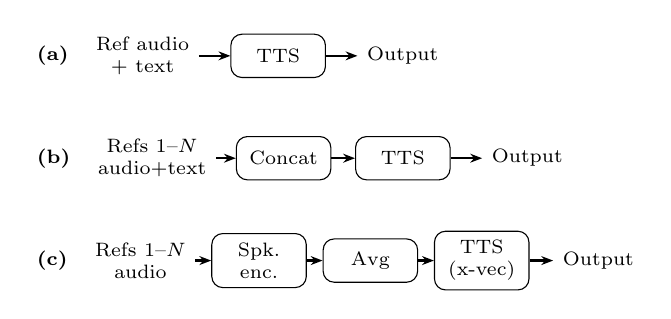
\begin{tikzpicture}[
    node distance=0.4cm and 0.5cm,
    box/.style={draw, rounded corners, minimum height=0.55cm, minimum width=1.2cm, font=\scriptsize, align=center},
    io/.style={font=\scriptsize, align=center},
    arr/.style={-{Stealth[length=1.5mm]}, thick},
    lbl/.style={font=\scriptsize\bfseries, anchor=west},
  ]
  % (a) Single baseline
  \node[lbl] (la) at (0, 0) {(a)};
  \node[io, right=0.1cm of la] (refa) {Ref audio\\+ text};
  \node[box, right=0.4cm of refa] (ttsa) {TTS};
  \node[io, right=0.4cm of ttsa] (outa) {Output};
  \draw[arr] (refa) -- (ttsa);
  \draw[arr] (ttsa) -- (outa);

  % (b) Audio concatenation
  \node[lbl] (lb) at (0, -1.3) {(b)};
  \node[io, right=0.1cm of lb] (ref1b) {Refs 1--$N$\\audio+text};
  \node[box, right=0.25cm of ref1b] (catb) {Concat};
  \node[box, right=0.3cm of catb] (ttsb) {TTS};
  \node[io, right=0.4cm of ttsb] (outb) {Output};
  \draw[arr] (ref1b) -- (catb);
  \draw[arr] (catb) -- (ttsb);
  \draw[arr] (ttsb) -- (outb);

  % (c) Embedding averaging
  \node[lbl] (lc) at (0, -2.6) {(c)};
  \node[io, right=0.1cm of lc] (ref1c) {Refs 1--$N$\\audio};
  \node[box, right=0.2cm of ref1c] (enc) {Spk.\\enc.};
  \node[box, right=0.2cm of enc] (avg) {Avg};
  \node[box, right=0.2cm of avg] (ttsc) {TTS\\(x-vec)};
  \node[io, right=0.3cm of ttsc] (outc) {Output};
  \draw[arr] (ref1c) -- (enc);
  \draw[arr] (enc) -- (avg);
  \draw[arr] (avg) -- (ttsc);
  \draw[arr] (ttsc) -- (outc);
\end{tikzpicture}%
}
\caption{Multi-reference voice cloning strategies.
(a)~Single baseline: one reference.
(b)~Audio concatenation: references concatenated as in-context examples.
(c)~Embedding averaging: embeddings averaged into one x-vector.}
\label{fig:method}
\end{figure}

\subsection{Experimental setup}
\label{sec:setup}

\textbf{Model.}
We use Qwen3-TTS-12Hz-0.6B-Base~\cite{qwen3tts} in bfloat16 precision on an NVIDIA A10G GPU (24\,GB VRAM).
To validate that conclusions are not idiosyncratic to this model size, we additionally repeat the experiment on Qwen3-TTS-12Hz-1.7B-Base (Section~\ref{sec:scale}).

\textbf{Dataset.}
Evaluation uses LibriTTS-R~\cite{libritts_r}, a restored version of LibriTTS~\cite{libritts}, at 24\,kHz.
We select 5 speakers (IDs: 1188, 1995, 4446, 4992, 5142), allocating 35 reference utterances and 5 held-out target texts per speaker.

\textbf{Experimental design.}
We vary: approach $\in \{\text{single, \textsc{concat}, \textsc{embed}}\}$, number of references $n \in \{1,2,3,5\}$, selection strategy $\in \{\text{random, longest}\}$, and random seed $\in \{42, 123, 456\}$.
This yields $5 \times 5 \times 3 \times 17 = 1{,}275$ synthesis runs (1~baseline + 8~\textsc{concat} + 8~\textsc{embed} configurations).

\subsection{Evaluation metrics}
\label{sec:metrics}

\textbf{Speaker similarity (SIM).}
Cosine similarity between WavLM-based speaker embeddings~\cite{wavlm} of synthesised and ground-truth speech, using the \texttt{wavlm-base-plus-sv} model.
We use an external speaker verification model rather than Qwen3-TTS's internal speaker encoder to avoid biasing SIM in favour of the embedding-averaging approach.

\textbf{Naturalness (UTMOS).}
Predicted mean opinion score from the UTMOS model~\cite{utmos}, an automated proxy for human naturalness judgments.

\textbf{Word error rate (WER).}
Whisper-turbo~\cite{whisper} transcription of synthesised audio compared to target text.
Because ASR error is non-negligible on ground-truth LibriTTS-R audio, we treat WER primarily as a stability proxy and report calibrated interpretation in Section~\ref{sec:significance}.

\textbf{Latency.}
Wall-clock synthesis time per utterance (excluding evaluation), including reference preprocessing and prompt construction, recorded as \texttt{tts\_time\_s}.

\textbf{Statistical testing.}
All comparisons use paired Wilcoxon signed-rank tests with Bonferroni correction ($\alpha = 0.05$, 48~comparisons).
We choose this non-parametric paired test because metric deltas can be heavy-tailed (especially WER), and apply Bonferroni to control family-wise error across configurations.
Effect sizes are reported as paired Cohen's $d_z$ computed on paired differences~\cite{cohen1988}.

%----------------------------------------------------------------------
\section{Results}
\label{sec:results}
%----------------------------------------------------------------------

\subsection{Overall comparison}
\label{sec:overall}

Table~\ref{tab:main} presents the full results.
\textsc{Concat} with the longest-reference strategy achieves the highest speaker similarity (SIM\,$=$\,0.949 at $n{=}3$), an improvement of $+$0.021 over the single baseline (0.928).
\textsc{Embed} achieves the highest naturalness (UTMOS\,$=$\,4.483 at $n{=}3$, random), an improvement of $+$0.058 over the baseline (4.425).
Neither approach simultaneously improves both metrics: \textsc{concat} maintains baseline-level naturalness while improving fidelity, and \textsc{embed} maintains baseline-level similarity while improving naturalness.

\begin{table*}[t]
\centering
\caption{Main results across all configurations.
Bold indicates best value per metric.
$\dagger$~Significant improvement over baseline ($p<0.05$, Bonferroni-corrected Wilcoxon signed-rank).}
\label{tab:main}
\small
\begin{tabular}{llcccc}
\toprule
\textbf{Approach} & \textbf{Strategy} & \textbf{\#Refs} & \textbf{UTMOS} $\uparrow$ & \textbf{Speaker SIM} $\uparrow$ & \textbf{WER (\%)} $\downarrow$ \\
\midrule
Single Baseline & random & 1 & 4.425 \scriptsize{$\pm$ 0.094} & 0.928 \scriptsize{$\pm$ 0.044} & 15.3 \scriptsize{$\pm$ 12.0} \\
\midrule
\textsc{Concat} & longest & 1 & 4.390 \scriptsize{$\pm$ 0.168} & 0.942 \scriptsize{$\pm$ 0.039} & 22.3 \scriptsize{$\pm$ 22.1} \\
\textsc{Concat} & random  & 1 & 4.431 \scriptsize{$\pm$ 0.119} & 0.926 \scriptsize{$\pm$ 0.047} & 15.9 \scriptsize{$\pm$ 12.7} \\
\textsc{Concat} & longest & 2 & 4.366 \scriptsize{$\pm$ 0.392} & 0.947$^\dagger$ \scriptsize{$\pm$ 0.036} & 24.1 \scriptsize{$\pm$ 73.6} \\
\textsc{Concat} & random  & 2 & 4.432 \scriptsize{$\pm$ 0.126} & 0.937 \scriptsize{$\pm$ 0.042} & 14.4 \scriptsize{$\pm$ 11.1} \\
\textsc{Concat} & longest & 3 & 4.416 \scriptsize{$\pm$ 0.098} & \textbf{0.949}$^\dagger$ \scriptsize{$\pm$ 0.038} & 21.3 \scriptsize{$\pm$ 18.0} \\
\textsc{Concat} & random  & 3 & 4.390 \scriptsize{$\pm$ 0.379} & 0.941 \scriptsize{$\pm$ 0.044} & 81.6 \scriptsize{$\pm$ 555} \\
\textsc{Concat} & longest & 5 & 4.400 \scriptsize{$\pm$ 0.143} & 0.948$^\dagger$ \scriptsize{$\pm$ 0.037} & 15.7 \scriptsize{$\pm$ 13.0} \\
\textsc{Concat} & random  & 5 & 4.385 \scriptsize{$\pm$ 0.381} & 0.944$^\dagger$ \scriptsize{$\pm$ 0.044} & 39.7 \scriptsize{$\pm$ 230} \\
\midrule
\textsc{Embed} & longest & 1 & 4.470$^\dagger$ \scriptsize{$\pm$ 0.086} & 0.936 \scriptsize{$\pm$ 0.037} & \textbf{13.4} \scriptsize{$\pm$ 10.4} \\
\textsc{Embed} & random  & 1 & 4.462$^\dagger$ \scriptsize{$\pm$ 0.082} & 0.921 \scriptsize{$\pm$ 0.045} & 14.5 \scriptsize{$\pm$ 11.6} \\
\textsc{Embed} & longest & 2 & 4.474$^\dagger$ \scriptsize{$\pm$ 0.087} & 0.934 \scriptsize{$\pm$ 0.040} & 14.0 \scriptsize{$\pm$ 10.8} \\
\textsc{Embed} & random  & 2 & 4.473$^\dagger$ \scriptsize{$\pm$ 0.072} & 0.927 \scriptsize{$\pm$ 0.042} & 13.8 \scriptsize{$\pm$ 11.3} \\
\textsc{Embed} & longest & 3 & 4.469$^\dagger$ \scriptsize{$\pm$ 0.078} & 0.939 \scriptsize{$\pm$ 0.037} & 15.0 \scriptsize{$\pm$ 13.6} \\
\textsc{Embed} & random  & 3 & \textbf{4.483}$^\dagger$ \scriptsize{$\pm$ 0.055} & 0.930 \scriptsize{$\pm$ 0.039} & 14.5 \scriptsize{$\pm$ 11.0} \\
\textsc{Embed} & longest & 5 & 4.474$^\dagger$ \scriptsize{$\pm$ 0.054} & 0.938 \scriptsize{$\pm$ 0.034} & 14.4 \scriptsize{$\pm$ 11.9} \\
\textsc{Embed} & random  & 5 & 4.463$^\dagger$ \scriptsize{$\pm$ 0.103} & 0.937 \scriptsize{$\pm$ 0.035} & 14.1 \scriptsize{$\pm$ 11.4} \\
\bottomrule
\end{tabular}
\end{table*}

\subsection{Statistical significance}
\label{sec:significance}

Table~\ref{tab:sig} summarises the significant results after Bonferroni correction.
For speaker similarity, four \textsc{concat} configurations achieve significance ($p < 0.003$, $d = 0.38$--$0.62$), three with the longest strategy and one with random.
The strongest effects appear with 3 and 5 references ($d = 0.60$ and $0.62$).

For naturalness, all eight \textsc{embed} configurations achieve significance ($p < 0.004$, $d = 0.32$--$0.61$).
The strongest effect is \textsc{embed} with 3 random references ($p < 10^{-7}$, $d = 0.61$).

No configuration produces a statistically significant change in WER after correction.
Whisper calibration on the 25 ground-truth target audios yields $\mathrm{WER}_{\text{GT}}=14.3\%$ median (IQR: $6.5$--$22.2\%$), indicating substantial ASR floor error unrelated to synthesis quality.
Accordingly, we interpret WER deltas conservatively and focus on catastrophic-failure rates.
\textsc{Embed} exhibits 0\% failures under this threshold across all tested configurations.
\textsc{Concat} is less stable, with failures across several settings (0--8\%) and the highest failure rate at $n{=}3$ with the longest strategy.
Random selection at $n{=}3$ additionally produces rare extreme outliers, inflating mean and variance (Table~\ref{tab:main}).

\begin{table}[t]
\centering
\caption{Statistically significant improvements over single baseline (Bonferroni-corrected Wilcoxon, $\alpha{=}0.05$).}
\label{tab:sig}
\small
\begin{tabular}{lclcc}
\toprule
\textbf{Config} & $n$ & \textbf{Metric} & $p_\text{corr}$ & $d$ \\
\midrule
\textsc{Concat}, long. & 2 & SIM & .002 & 0.51 \\
\textsc{Concat}, long. & 3 & SIM & $<$.001 & 0.60 \\
\textsc{Concat}, long. & 5 & SIM & $<$.001 & 0.62 \\
\textsc{Concat}, rand. & 5 & SIM & .002 & 0.38 \\
\midrule
\textsc{Embed}, long. & 1 & UTMOS & $<$.001 & 0.43 \\
\textsc{Embed}, rand. & 1 & UTMOS & .004 & 0.36 \\
\textsc{Embed}, long. & 2 & UTMOS & $<$.001 & 0.46 \\
\textsc{Embed}, rand. & 2 & UTMOS & $<$.001 & 0.50 \\
\textsc{Embed}, long. & 3 & UTMOS & $<$.001 & 0.45 \\
\textsc{Embed}, rand. & 3 & UTMOS & $<$.001 & 0.61 \\
\textsc{Embed}, long. & 5 & UTMOS & $<$.001 & 0.55 \\
\textsc{Embed}, rand. & 5 & UTMOS & $<$.001 & 0.32 \\
\bottomrule
\end{tabular}
\end{table}

\subsection{Pareto trade-off}
\label{sec:scaling}

Figure~\ref{fig:scaling} visualises the main result directly in SIM--UTMOS space.
\textsc{Concat}+longest occupies the high-SIM frontier (peak SIM at $n{=}3$), while \textsc{embed} occupies the high-UTMOS frontier (peak UTMOS at $n{=}3$, random).
No configuration dominates both axes, confirming the Pareto trade-off and motivating task-specific operating-point selection.

\begin{figure}[t]
  \centering
  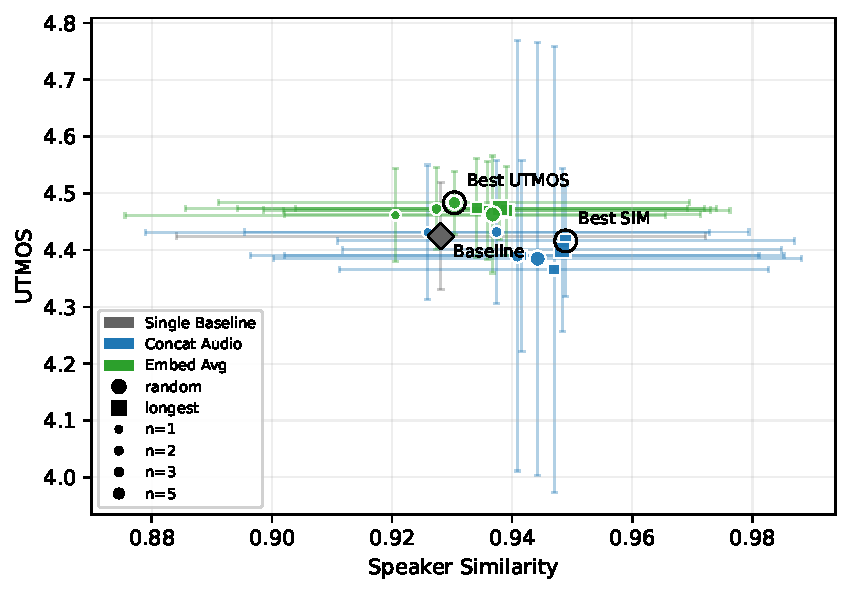
\includegraphics[width=\columnwidth]{figures/pareto_tradeoff}
  \caption{Pareto trade-off between speaker similarity and naturalness across configurations (means with $\pm$1~SD).
  \textsc{Concat}+longest maximises SIM, while \textsc{embed} maximises UTMOS.}
  \label{fig:scaling}
\end{figure}

\subsection{Scaling with number of references}
\label{sec:scaling_curve}

Figure~\ref{fig:scaling_curve} shows average performance as the number of references increases.
Both approaches exhibit diminishing returns beyond $n{=}3$, supporting the practical guideline that reference quality and selection strategy matter more than adding additional short references.

\begin{figure}[t]
  \centering
  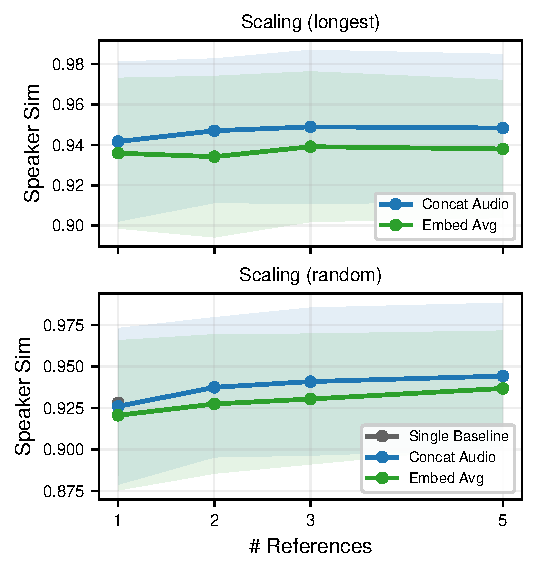
\includegraphics[width=\columnwidth]{figures/scaling_curve}
  \caption{Scaling with reference count. Both SIM and UTMOS improvements plateau beyond $n{=}3$ for the tested strategies.}
  \label{fig:scaling_curve}
\end{figure}

\subsection{Reference selection strategy}
\label{sec:strategy}

Figure~\ref{fig:strategy} shows stability through catastrophic-failure rates.
The instability risk is specific to \textsc{concat} configurations.
The highest failure rate under WER$>50\%$ occurs for \textsc{concat}+longest at $n{=}3$, while random selection exhibits the heaviest tail (Table~\ref{tab:main}).
These failures also manifest as latency spikes: on 0.6B, synthesis time (median/p95/max) is 8.2/31.9/40.1\,s (baseline), 8.0/37.4/41.9\,s (\textsc{concat}+longest, $n{=}3$), and 8.9/35.2/36.3\,s (\textsc{embed}+random, $n{=}3$), while \textsc{concat}+random at $n{=}3$ reaches 297.8\,s in the worst case.

For \textsc{embed}, the impact of selection strategy is smaller and inconsistent, aligning with the interpretation that embedding extraction is less sensitive to utterance duration than in-context processing.

\begin{figure}[t]
  \centering
  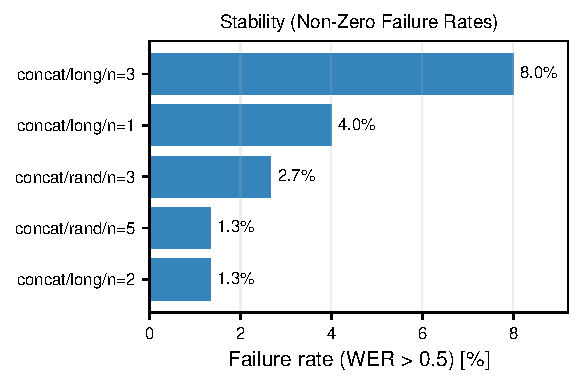
\includegraphics[width=\columnwidth]{figures/stability_fail_rate}
  \caption{Stability analysis using catastrophic failure rate (WER$>50\%$).
  Only configurations with non-zero failure rates are shown.
  Failures occur only in \textsc{concat} settings: the highest failure rate is \textsc{concat}+longest at $n{=}3$, while \textsc{concat}+random exhibits rarer but more extreme outliers.}
  \label{fig:strategy}
\end{figure}

\subsection{Per-speaker analysis}
\label{sec:perspeaker}

The fidelity--naturalness trade-off is consistent across all 5~speakers, though magnitude varies.
Notably, preliminary single-speaker experiments on one speaker initially suggested \textsc{embed} dominance across both metrics---a finding that did not generalise to the full 5-speaker evaluation.
This highlights the importance of multi-speaker testing for drawing reliable conclusions about voice cloning strategies.

\subsection{Model scale validation}
\label{sec:scale}

To test whether the Pareto trade-off persists with model scale, we repeat the full experiment on Qwen3-TTS-1.7B.
Results are qualitatively consistent.
\textsc{Concat}+longest improves speaker similarity (0.932 to 0.948 at $n{=}3$, $p_\text{corr}{=}5.0e-4$, $d{=}0.57$), while \textsc{embed}+random improves naturalness (4.453 to 4.491 at $n{=}3$, $p_\text{corr}{=}6.5e-7$, $d{=}0.60$).
This suggests the trade-off is robust within the Qwen3-TTS family across at least two model sizes.

\subsection{Exploratory perceptual probe (qualitative)}
\label{sec:perceptual}

A small exploratory blind comparison (1~listener, 4~paired comparisons) was conducted to qualitatively probe alignment between automated metrics and human perception.
The listener preferred \textsc{concat} for speaker identity and \textsc{embed} for naturalness, broadly aligning with automated results on the naturalness axis.
However, in one case where the SIM metric favoured \textsc{embed} (0.983 vs.\ 0.976), the listener judged \textsc{concat} as the better voice match.
While far too limited for statistical inference, this observation suggests that cosine similarity in WavLM embedding space may not fully capture perceptual voice identity.
A statistically powered listener study is required to assess perceptual significance.

%----------------------------------------------------------------------
\section{Discussion and Conclusion}
\label{sec:conclusion}
%----------------------------------------------------------------------

We have presented a systematic comparison of two multi-reference voice cloning strategies for Qwen3-TTS across 1{,}275~controlled synthesis runs.
Our central finding is a Pareto trade-off: audio concatenation optimises speaker fidelity ($d$ up to $0.62$), while embedding averaging optimises naturalness ($d$ up to $0.61$), with neither dominating both objectives.

This trade-off has practical implications.
For applications prioritising speaker fidelity---as reflected by SIM---\textsc{concat} with longest references at $n{=}3$ may be preferred.
For applications prioritising naturalness---virtual assistants, accessibility tools---\textsc{embed} offers more natural output with stable performance regardless of reference count or selection strategy.
Notably, \textsc{embed} uses the model's \texttt{x\_vector\_only} conditioning pathway, whereas single and \textsc{concat} use prompt-based conditioning. The fact that \textsc{embed} achieves significant UTMOS improvement already at $n{=}1$ (before any averaging occurs) strongly suggests the naturalness gain is primarily attributable to the conditioning pathway rather than multi-reference averaging. This is an important confound: our results characterise the two strategies as deployed, but cannot isolate the averaging effect from the conditioning mode effect.

Our scaling analysis reveals that reference selection strategy (longest vs.\ random) matters more than the number of references beyond~3.
Results suggest practitioners may benefit from prioritising high-quality, longer reference utterances over accumulating additional references.

The pilot perceptual evaluation raises important questions about the validity of embedding-cosine speaker similarity as an evaluation metric.
If automated SIM diverges from human perception, improvements measured in embedding space may not directly translate to perceived quality gains.
Formal listening tests with crowdsourced evaluators are needed to assess this.

\textbf{Limitations.}
We evaluate one TTS architecture family (Qwen3-TTS) at two model sizes (0.6B and 1.7B) on a single dataset (LibriTTS-R) in English only.
Generalisability to other models (e.g., VALL-E~\cite{valle}, CosyVoice~\cite{cosyvoice}), languages, and acoustic conditions remains to be established.
The perceptual evaluation is preliminary ($n{=}1$) and requires validation with a statistically powered listener panel.
The perceptual probe is qualitative only and does not permit statistical conclusions about listener preference or perceptual effect size.

\textbf{Future work.}
We plan to extend this comparison to additional TTS architectures and model sizes, conduct crowdsourced MOS and speaker similarity evaluations, explore hybrid strategies combining both approaches, and investigate cross-lingual multi-reference cloning.

\textbf{Reproducibility.}
Code and samples will be made available upon publication.

\clearpage
\section*{Generative AI Use Disclosure}
A generative AI coding assistant was used for experiment scripting and manuscript preparation.
All results, analysis, and scientific claims were verified by the authors.

%----------------------------------------------------------------------
% References
%----------------------------------------------------------------------

\bibliographystyle{IEEEtran}
\bibliography{refs}

\end{document}
